\documentclass[conference]{IEEEtran}
\IEEEoverridecommandlockouts
\usepackage[utf8]{inputenc}
\usepackage[T1]{fontenc}
\usepackage{amsmath,amssymb}
\usepackage{graphicx}
\usepackage{booktabs}
\usepackage{url}
\usepackage[hidelinks]{hyperref}
\graphicspath{{figures/}}

\begin{document}

\title{Benchmark and Oracle Reliability in Evaluating Semantic Change Detection for Legacy Software: A Negative Empirical Study}

\author{\IEEEauthorblockN{Anonymous Submission}
\IEEEauthorblockA{Author details withheld for double-blind review}}

\maketitle

\begin{abstract}
Legacy batch systems encode behaviour in job control language (JCL), where small edits can change outcomes silently. Semantic change detectors promise to flag such edits, but their evaluations rest on benchmark labels and oracle assumptions that are seldom audited. We study RELIC V2, a static JCL contract analyser, against a normalized text-diff baseline on JCL-SemBench (180 pairs) and on an external run of 824 mutants, of which 7 of the 11 listed repositories contribute evaluable mutants. A pre-specified comparison rejects the hypothesis that RELIC V2 beats the normalized text baseline: MCC is 0.324 against 0.525 (paired difference $-0.20$, 95\% cluster-bootstrap CI $[-0.30,-0.10]$). RELIC V2 detects no changing case that the baseline misses in any population. Our audit found 15 of 93 changing pairs byte-identical, 13 oracle disagreements, and 21 groups of duplicated pairs; all five groups with contradictory labels consist of byte-identical pairs. Post hoc exclusions move the MCC gap between $-0.12$ and $-0.33$. External labels are almost fully determined by mutation operator: one operator rule matches 821 of 824 labels. We found no measurable value from the semantic layer over a simple baseline, and we show that benchmark construction alone can change the conclusion. No human validation, held-out corpus or independent oracle was available, so all evidence is development or same-author evidence.
\end{abstract}

\begin{IEEEkeywords}
legacy modernisation, job control language, semantic change detection, benchmark construction, test oracles, negative results, responsible evaluation
\end{IEEEkeywords}

\section{Introduction}
Mainframe batch jobs written in JCL sequence programs, datasets and return-code guards. Re-implementing or refactoring them can alter behaviour without any visible failure, and the obligations behind a job are rarely written down. Automated analysis that flags behaviour-changing edits is therefore attractive for legacy modernisation.

RELIC V2 is a static analyser that extracts job-level contracts (temporal ordering, dataset resources and conditional control flow) and reports the contracts a change breaks. Its appeal is that it names the violated contract, which a textual check cannot. The question that matters is whether this added semantic structure detects more real changes than a cheap rule, and whether the benchmark can tell the two apart.

We report a negative empirical study. We do not claim RELIC V2 fails in general. We show that, on the available evidence, its semantic layer adds no measurable detection capability over a normalized text diff, and that benchmark and oracle choices materially change the reported comparison. Our contributions are: (i) a pre-specified comparison with a normalized text baseline on two benchmarks; (ii) an error-overlap analysis showing zero RELIC-only true positives; (iii) a benchmark and oracle audit with sensitivity analyses; and (iv) reporting practices for evaluating semantic analysers, tied to responsible evaluation.

\section{Background and Motivation}
JCL jobs are sequences of steps. A step runs a program with dataset disposition (DISP) and condition (COND) parameters, and later steps depend on datasets written by earlier ones. A change such as moving a consumer before its producer, altering a disposition or removing a return-code guard can change which datasets exist and which steps run, without touching program text.

Mutation analysis is a standard way to build labelled change benchmarks, but it has known validity problems: mutants are not representative faults, and equivalent or redundant mutants distort scores~\cite{andrews2005,jia2011,papadakis2016}. Equivalent-mutant judgement is now delegated to language models~\cite{tian2024}, and LLM-based legacy analysis has been reported for COBOL and PL/I~\cite{kalohia2026}. Static COBOL control-flow work exists~\cite{deknop2022}, and semantic change validation has been studied for Python~\cite{changeguard2025}. We found no peer-reviewed evaluation of JCL contract checking against an execution-semantics oracle. Our search was incomplete, and commercial tools and patents cover JCL dependency extraction, which we do not evaluate.

\section{Research Questions}
\begin{description}
\item[RQ1] Does RELIC V2 detect behaviour-changing JCL edits more accurately than a normalized text-diff baseline?
\item[RQ2] Does RELIC V2 detect any changing case that the text baseline misses?
\item[RQ3] How sensitive are the comparison's conclusions to benchmark construction and label quality?
\end{description}
The decision rules for RQ1 and RQ2 were written into a pre-registration file after the aggregate results were known. They are therefore not confirmatory tests. We state the rules in advance and treat everything else as exploratory.

\section{Methodology}
Figure~\ref{fig:pipeline} separates the evidence by status. Development and external results both come from the same author's oracle, and neither is blind or held out.

\begin{figure*}[t]
\centering
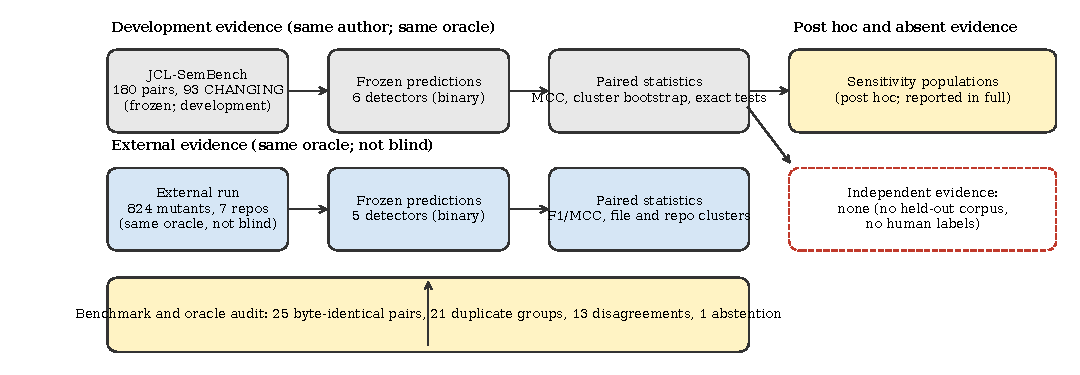
\includegraphics[width=\textwidth]{fig0_evaluation_pipeline.pdf}
\caption{Evaluation pipeline and evidence status. Grey: development evidence (JCL-SemBench). Blue: external evidence (same oracle, not blind). Yellow: post hoc analyses and the audit. Red dashed: independent evidence, which does not exist for RELIC V2.}
\label{fig:pipeline}
\end{figure*}

\subsection{Subjects and detectors}
JCL-SemBench contains 180 original-and-transformed JCL pairs, 93 labelled CHANGING and 87 PRESERVING, drawn from 16 base programs. Each label is the benchmark author's expectation, checked against a separately written execution-semantics model (the oracle). The oracle shares no code with RELIC V2 but has the same author. The external run takes mutants from 11 listed public repositories. Under the frozen scope, 824 are evaluable, and 589 of them come from one repository (\texttt{yetacp\_mvs\_sysgen}). The external run uses the same oracle and was not blind.

Detectors are binary and emit no score. RELIC V2 flags a pair when its contract diff is non-empty. The primary text baseline on SemBench is \texttt{normalized\_text\_B}, which strips comments, joins continuations, collapses whitespace, ignores case outside quotes and sorts keyword operands. On the external run the frozen comparator is \texttt{textdiff\_ignore\_job\_parameters}, which also ignores JOB-card parameters. Plain text diff and a raw-text variant are reference points. Text baseline code was hash-recorded before the external run.

\subsection{Statistics}
Proportions carry Wilson 95\% intervals. MCC and F1 intervals are percentile cluster bootstraps with 10{,}000 resamples and seed 20261004, clustered on \texttt{base\_id} (SemBench, 16 clusters) and on source file (external, 71 clusters). Repository-clustered intervals (7 clusters) are descriptive only. Paired comparisons use exact McNemar tests, an exact cluster sign-flip test and Holm correction. Holm p-values depend on how many tests are counted, so we report three families (14, 56 and 86 tests). An independent script recomputed every reported number from the raw prediction files, and all published values reproduced.

\subsection{Benchmark and oracle audit}
We checked byte equality of each original and transformed file, groups of duplicated pairs and their labels, oracle agreement with each stated expectation, and the frozen manifest.

\section{Results}
\subsection{RQ1: accuracy against the text baseline}
Table~\ref{tab:main} gives the direct comparisons. On SemBench, RELIC V2 has high precision (0.920; 23 of 25 flags correct) but low recall (0.247). The text baseline reaches recall 0.839 at precision 0.736. The paired MCC difference is $-0.201$ (95\% CI $[-0.299,-0.102]$), so the pre-registered rule rejects H1 (RELIC V2 has higher MCC than the baseline). Table~\ref{tab:sens} shows the same direction in every population.

The Holm-adjusted $p$ for this pair depends on which tests are corrected together. It is $p=0.020$ for the published 14-test family, $0.029$ across the 27 distinct tests the repository published, and $0.054$ across the 42 distinct tests our reanalysis ran. Identical tests are collapsed in both cases. The pre-registered comparator is normalized text B. Against normalized text A (B without keyword-operand sorting, which differs from B on seven cases) the MCC difference is $-0.127$ [$-0.219$, $-0.033$], so the bootstrap rule also rejects H1 there; its raw McNemar $p$ is $0.025$ and it does not survive Holm correction over 86 tests. Against plain text diff, RELIC V2 is \emph{better} in MCC ($+0.148$ [$+0.038$, $+0.247$]), because plain text diff flags 60 of the 87 PRESERVING pairs. Against the text diff that ignores JOB parameters the difference is a tie ($+0.022$ [$-0.077$, $0.120$]). RELIC V2 is therefore beaten by the normalizing text rules but not by every text rule. H1 rests on the bootstrap rule, not on Holm.

On the external run RELIC V2 has precision 1.000 and recall 0.952. The frozen text comparator has recall 1.000 and precision 0.996. The pooled F1 difference is $-0.022$ (file-cluster 95\% CI $[-0.042,-0.008]$). Repository-clustered intervals include zero ($[-0.032,0.004]$). Excluding the repository that supplies 71.5\% of mutants, the two detectors are indistinguishable (F1 difference $-0.005$ [$-0.027$, $0.010$]; MCC difference $-0.027$ [$-0.124$, $0.060$]).

The per-case McNemar test does not match the hypothesis. Its discordant pairs split by class: every case the baseline catches and RELIC misses is CHANGING, and every case RELIC gets right and the baseline gets wrong is PRESERVING. Its verdict therefore tracks class balance rather than MCC. Against plain text diff, for example, the MCC difference is $+0.148$ while McNemar gives $p=0.85$. We use the paired cluster-bootstrap MCC difference as the primary test and report McNemar only as secondary.

\begin{table}[t]
\caption{Pre-registered hypotheses and verdicts. Rules were written after the results were known, so these verdicts are post hoc applications of stated rules.}
\label{tab:hyp}
\centering
\small
\resizebox{\columnwidth}{!}{\begin{tabular}{@{}p{0.30cm}p{4.3cm}p{2.5cm}@{}}
\toprule
ID & Rule and evidence & Verdict \\
\midrule
H1 & RELIC V2 has higher MCC than normalized text B (SemBench, all pairs). $\Delta$MCC $-0.201$ [$-0.299$, $-0.102$] & Rejected \\
H2 & RELIC detects changes the text baseline misses. RELIC-only true positives: 0 in every population & Rejected \\
H3 & External precision $\geq 0.95$. Pooled 658/658; lowest per-repository Wilson lower bound 0.912 (file-level, unclustered) & Not rejected \\
H4 & Fast-track avoids $\geq 30\%$ of reviews at $\leq 1\%$ wrongly accepted. SemBench 23.6--25.0\% avoided; external 94.8\%, not blind & Rejected on SemBench; met on external \\
H5 & Explanations name the violated contract. Not testable from binary flags & Untested \\
\bottomrule
\end{tabular}}
\end{table}

\begin{table}[t]
\caption{Direct experimental comparisons. Brackets give 95\% cluster-bootstrap intervals for MCC (SemBench: 16 base programs; external: 71 files). Literature-reported figures are not comparable and are not shown.}
\label{tab:main}
\centering
\small
\resizebox{\columnwidth}{!}{\begin{tabular}{@{}llcccc@{}}
\toprule
Method & Benchmark & Prec. & Rec. & F1 & MCC [95\%] \\
\midrule
RELIC V2 & SemBench (180) & 0.920 & 0.247 & 0.390 & 0.324 [0.248, 0.382] \\
Normalized text (B) & SemBench (180) & 0.736 & 0.839 & 0.784 & 0.525 [0.420, 0.629] \\
RELIC V2 & External (824) & 1.000 & 0.952 & 0.976 & 0.874 [0.807, 0.937] \\
Normalized text (ignore JOB) & External (824) & 0.996 & 1.000 & 0.998 & 0.987 [0.965, 1.000] \\
Plain text diff & External (824) & 0.918 & 1.000 & 0.957 & 0.700 [0.675, 0.725] \\
\bottomrule
\end{tabular}}
\end{table}

\subsection{RQ2: zero complementary detections}
In every SemBench population and in the external run, RELIC V2 has no true positive that the text baseline misses. On the 93 changing SemBench cases, both detect 23, the text baseline alone detects 55 and 15 are missed by both (Fig.~\ref{fig:main}b). All 15 are byte-identical pairs labelled CHANGING, so no detector can catch them. RELIC V2's flagged set is a strict subset of the text baseline's flagged set on both classes. Its only advantage is 26 correct rejections of harmless edits that the baseline flags. We do not conclude the semantic layer is useless. The data show only that it adds no detections here.

\subsection{RQ3: sensitivity to benchmark construction}
Table~\ref{tab:sens} shows how the same comparison changes under the benchmark's own defects. Excluding the 25 byte-identical pairs widens the gap, because the 15 CHANGING no-ops are missed by every detector and therefore depress the high-recall text baseline. Excluding the 13 oracle disagreements roughly halves the gap, and RELIC V2 then has no false positives. These exclusions are post hoc sensitivity analyses on the same data, not new confirmatory tests, and we report all of them.

\begin{table}[t]
\caption{Sensitivity of the SemBench MCC difference (RELIC V2 minus normalized text B). Paired cluster bootstrap, 10{,}000 resamples. Negative values favour the text baseline. Exclusions after the first row are post hoc.}
\label{tab:sens}
\centering
\small
\resizebox{\columnwidth}{!}{\begin{tabular}{@{}lccc@{}}
\toprule
Population & Changing n & $\Delta$MCC [95\%] & Clusters \\
\midrule
All pairs (pre-registered) & 93 & $-0.201$ [$-0.299$, $-0.102$] & 16 \\
Excl.\ 15 byte-identical CHANGING & 78 & $-0.328$ [$-0.435$, $-0.245$] & 16 \\
Excl.\ 25 byte-identical & 78 & $-0.319$ [$-0.431$, $-0.230$] & 16 \\
Clean core (no identical/disputed) & 67 & $-0.230$ [$-0.370$, $-0.129$] & 16 \\
Excl.\ 13 oracle disagreements & 83 & $-0.123$ [$-0.239$, $-0.022$] & 16 \\
\bottomrule
\end{tabular}}
\end{table}

\section{Benchmark and Oracle Audit}
Figure~\ref{fig:comp} gives the mutually exclusive composition. Of the 180 pairs, 25 are byte-identical. Fifteen of these are labelled CHANGING, a generator error since the transformation was not applied. Thirteen pairs disagree with the oracle and one abstains. The generator has no assertion that the transformed file differs from the original. Five pairs labelled as consecutive step inversions are in fact appended steps. Grouping pairs by their original and transformed bytes gives 21 duplicate groups covering 46 cases. Nine of these groups consist of byte-identical pairs, and all five contradictory groups (the same bytes labelled both CHANGING and PRESERVING) are among them, so the contradictions are a consequence of the no-op defect rather than a separate problem. The remaining 12 groups (24 cases) are non-identical and have consistent labels. The 180 pairs come from only 16 distinct base programs. Of the 87 PRESERVING pairs, 46 are comment, whitespace/continuation or JOB-card edits, which the normalizer's rules target directly; it rejects 44 of these 46. Of the 41 structural negatives it rejects only 15.

On the external run the label is almost fully determined by operator. Predicting positive unless the operator is \texttt{INSERT\_COMMENT} or \texttt{CHANGE\_MSGCLASS} matches 821 of 824 labels, so external F1 and MCC measure recognition of non-cosmetic operators rather than behavioural reasoning, for RELIC V2 and the text baseline alike. Only three evaluable negatives are non-cosmetic. The frozen scope also excludes 163 \texttt{RENAME\_OUTPUT\_DATASET} mutants. The oracle labels 144 of these as changing, the text baseline catches all 144, and RELIC V2 catches 3. Adding them back in a post hoc analysis reduces RELIC V2's recall to 0.792 (F1 0.884), against 0.997 for the text comparator.

\begin{figure*}[t]
\centering
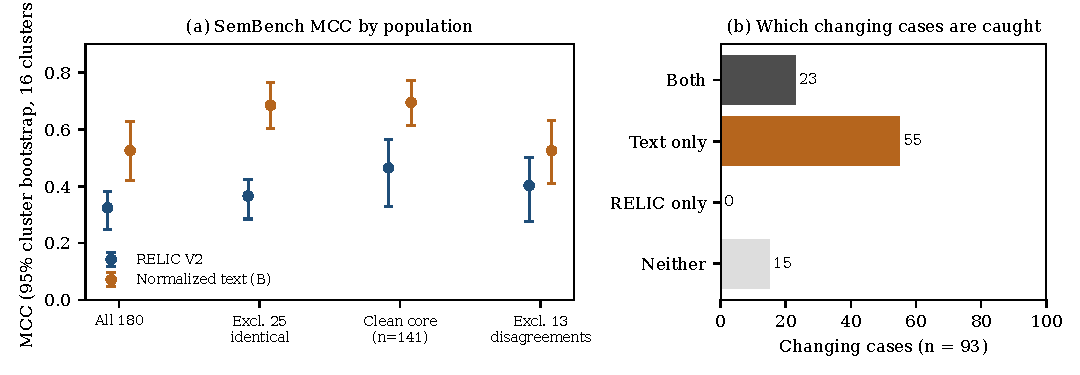
\includegraphics[width=\textwidth]{fig1_mcc_and_overlap.pdf}
\caption{(a) SemBench MCC for RELIC V2 and normalized text B across four populations, with 95\% cluster-bootstrap intervals (16 base programs). Populations after the first are post hoc. (b) Changing cases caught by each detector in the all-pairs population (n = 93): RELIC V2 catches no case that the text baseline misses.}
\label{fig:main}
\end{figure*}

\begin{figure}[t]
\centering
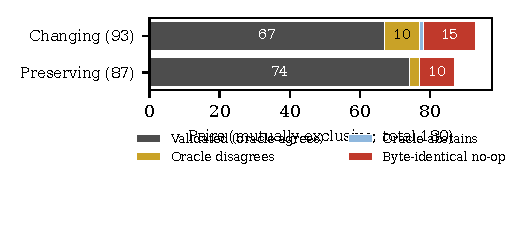
\includegraphics[width=\columnwidth]{fig2_benchmark_composition.pdf}
\caption{SemBench composition, mutually exclusive, computed from \texttt{cases.jsonl}. Byte-identical pairs are generator no-ops. Disagreements and abstentions are oracle outcomes.}
\label{fig:comp}
\end{figure}

\section{Discussion and Implications}
\textbf{Responsible experimental design.} The conclusion depends on which population is reported. Under the pre-registered population, RELIC V2 is clearly worse. After removing identical and disputed pairs, the gap shrinks but remains. On the external run the difference depends on the clustering level. A paper that reported only one view would give a different impression. We recommend that evaluations of semantic analysers publish every population and its exclusion rule, decided before results are seen.

\textbf{Data and label quality.} Byte-identical CHANGING pairs, duplicated and contradictory labels and oracle disagreements are not cosmetic. Here they change the magnitude of every sub-analysis. A benchmark that rewards text near-identity while penalising a detector for the same identity will mislead anyone choosing a tool.

\textbf{Baseline fairness and claims.} A normalized text diff is a strong, cheap baseline, and a semantic analyser should show measurable value over it before its extra machinery is justified. Our data give no such evidence for RELIC V2. The external comparator was chosen after the development benchmark's operator set was known, which we disclose. Negative operators there edit only comments or JOB parameters, so the comparator's rule matches the external labels by construction. A stronger hand-built text rule could test the baseline's cost more fairly, and we did not build one.

\textbf{Oracle accountability.} The oracle is code-independent of RELIC V2 but shares authorship, a lexer and a model with the mutator that creates the positives. Its labels are not externally validated. Calling it independent overstates its standing, so we use ``same-author, unvalidated'' throughout. An unvalidated oracle can make the same tool look better or worse depending on which disputed labels are kept.

\textbf{Responsible claims.} The narrow statement this study supports is that, on these benchmarks, a static JCL contract analyser did not outperform a normalized text diff and produced no detections the text diff lacked. Presenting its precision or its named contracts as a benefit without that context would overstate the evidence.

\section{Threats to Validity}
\textbf{Construct.} ``Changing'' is the benchmark author's expectation, checked by a same-author oracle. A different notion of behavioural change could reverse some labels. The detectors are binary, so we cannot report precision--recall curves or threshold analyses, and we do not evaluate explanation quality.

\textbf{Internal.} The benchmark author also wrote RELIC V2, the mutator, the oracle and the text baselines. Several text-baseline rules map one-to-one onto benchmark categories, so the baseline's advantage is partly built in. We could not verify when the rule author saw the taxonomy.

\textbf{External.} The external run is not blind and uses the same oracle. One repository supplies 71.5\% of evaluable mutants. Only seven of the eleven listed repositories contribute, and the provenance of that largest repository is not fully verified.

\textbf{Statistical conclusion.} With 16 base programs and 7 repositories, cluster bootstraps are unstable and may under-cover. The Holm figure for the SemBench headline ranges from $p=0.020$ (14-test family) through $0.029$ (27 distinct published tests) to $0.054$ (42 distinct tests in our reanalysis). H1 is decided by the bootstrap rule, not by the Holm $p$-value.

\section{Limitations}
This is a negative empirical study of one tool and two benchmarks. No held-out corpus exists: every subject was seen during development. No human has labelled any pair, so no oracle label is validated by a practitioner. Our review package of 60 cases has zero returned responses and is not validation. No language-model baseline was run because no API credentials were available, so the comparison with LLMs is untested. Post hoc exclusions and the scope-inclusive external analysis are sensitivity analyses, not confirmatory results. We do not claim generalisation to production JCL, to z/OS execution or to other languages.

\section{Conclusion}
We asked whether a semantic JCL contract analyser adds measurable detection value over a normalized text diff. On the available benchmarks it does not. The pre-registered MCC comparison favours the baseline, RELIC V2 finds no change the baseline misses, and the conclusion depends materially on benchmark construction and oracle labels. The lesson for responsible evaluation is that semantic analysers should show value over simple baselines on benchmarks whose labels have been audited, and that the audit should be reported. A held-out, independently labelled corpus is the necessary next step.

\section*{Reproducibility}
All numbers are computed from committed prediction files, the frozen benchmark manifest and scripts in the repository's recovery branch. Benchmark files are not modified. In a clean clone, the SemBench evaluation and the external run (cloned at the frozen commits) reproduced their committed predictions, metrics and paired tests byte-for-byte, and the full pipeline ran to completion. The Docker build did not reproduce. Figures are generated by a script from the analysis outputs. Repository identifiers are withheld for review and will be provided on acceptance.

\begin{thebibliography}{1}
\bibitem{andrews2005} J.~H. Andrews, L.~C. Briand, and Y.~Labiche, ``Is mutation an appropriate tool for testing experiments?'' in \emph{Proc. ICSE}, 2005, doi:10.1145/1062455.1062530.
\bibitem{jia2011} Y.~Jia and M.~Harman, ``An analysis and survey of the development of mutation testing,'' \emph{IEEE Trans. Softw. Eng.}, 2011, doi:10.1109/TSE.2010.62.
\bibitem{papadakis2016} M.~Papadakis, C.~Henard, M.~Harman, and Y.~Jia, ``Threats to the validity of mutation-based test assessment,'' in \emph{Proc. ISSTA}, 2016, doi:10.1145/2931037.2931040.
\bibitem{tian2024} Y.~Tian \emph{et al.}, ``Large language models for equivalent mutant detection: How far are we?'' in \emph{Proc. ISSTA}, 2024, doi:10.1145/3650212.3680395.
\bibitem{kalohia2026} A.~Kalohia, ``Leveraging generative AI for extracting business requirements from legacy COBOL and PL/I code,'' in \emph{Proc. ACL Industry Track}, 2026. \url{https://aclanthology.org/2026.acl-industry.4/}.
\bibitem{deknop2022} C.~Deknop, J.~Fabry, K.~Mens, and V.~Zaytsev, ``Generating customised control flow graphs for legacy languages with semi-parsing,'' in \emph{Proc. ICSME}, 2022, doi:10.1109/ICSME55016.2022.00072.
\bibitem{changeguard2025} L.~Gr\"oninger, B.~Souza, and M.~Pradel, ``ChangeGuard: Validating code changes via pairwise learning-guided execution,'' \emph{Proc. ACM Softw. Eng.}, 2025, doi:10.1145/3715760.
\end{thebibliography}

\end{document}
